\documentclass{article}

% Language setting
% Replace `english' with e.g. `spanish' to change the document language
\usepackage[english]{babel}

% Set page size and margins
% Replace `letterpaper' with `a4paper' for UK/EU standard size
\usepackage[letterpaper,top=2cm,bottom=2cm,left=3cm,right=3cm,marginparwidth=1.75cm]{geometry}

% Useful packages
\usepackage{amsmath}
\usepackage{graphicx}
\usepackage[colorlinks=true, allcolors=blue]{hyperref}

\title{Binocular depth perception}
\author{Ronak Agarwal}

\begin{document}
\maketitle

\begin{abstract}
\noindent Convolutional Neural Networks (CNN's), are being compared to human cognition (\href{https://doi.org/10.1371/journal.pcbi.1011086}{Bracci et al., 2023}). However, unlike classical CNNs, most humans have the benefit of two visual input sources (left and right eye). This allows human visual systems to determine depth using binocular cues, while CNNs are forced to rely on monocular heuristics. As depth perception is crucial in image analysis and object differentiation, this fundamental sensory difference is a big limitation in studies comparing monocular CNN's to the human visual cortex. \newline \newline
Long term, this project seeks to create a binocular CNN that can estimate depth, use mechanistic interpretability to determine how the algorithm estimates depth, and/or compare this new network to the human visual cortex. Currently, this project is an early-stage write-up of a potentially extensive research direction. I also analytically derive a method by which depth may be calculated for binocular inputs. 

\end{abstract}

\section{Introduction}

\indent This project has lots of limitations, unknowns, and difficult obstacles. Some include:
\begin{enumerate}
    \item If showing people 2D images, isn't that essentially not using their binocular depth perception?
    \item Humans and computer would have different binocular depth perception algorithms because of attention, prior world conception, object movement, ability to move eyes, etc. For example, humans might estimate depth by measuring the difference in eye-angle when focusing on an object, while a computer with stationary cameras would implement a different algorithm.
    \item Chicken vs egg in computer binocular depth perception vs object differentiation (discussed more later).
    \item And much more!
\end{enumerate}
Despite these limitations, this project communicates the general idea that when comparing human and AI cognition, the fundamental setup needs to align. This project doesn't match human and artificial cognitive architectures perfectly, but it helps closes the gap. While this project might not have perfect application, it seems fun to try, binocular CNN's seem like an interesting new thing to attempt to create, and the whole thing will be a cool learning experience. \newline \newline
Some high-level obstacles with binocular CNNs and difficulties comparing computer vision and the human visual cortex include:
\begin{enumerate}
    \item Object differentiation is required for depth perception, but depth perception helps with object differentiation: chicken or egg?
    \item  Maybe the system tries to move parameters in a direction that creates a consistent system between object differentiation and depth, but outlining this explicitly seems tough.
    \item Human vision also has the benefit of preconception, object conception, attention, etc. This might mean that the human visual cortex cognitive architecture will always be fundamentally different than CNN's, making it impossible to draw perfect comparisons between the two. 
\end{enumerate}



\section{Phase I}
The work on this problem was largely geometric, so I'll include images. Furthermore, I made some assumptions about cameras that could be incorrect/depend on the setup. \newline \newline
There were a couple different "algorithms" I could have tried to implement with binocular camera vision, and I went with how much an object location shifts between the two cameras. Intuitively, the further away an object is, the less it will appear to shift between the two cameras. \newline \newline
To follow the math I did, it's easier if all the quantities I used are given variables. The following image shows how I define the variables $p$, $q$, $l$, $d$, $a$, $b$, $\theta$, and $\phi$. 
\begin{figure}[htp]
    \centering
    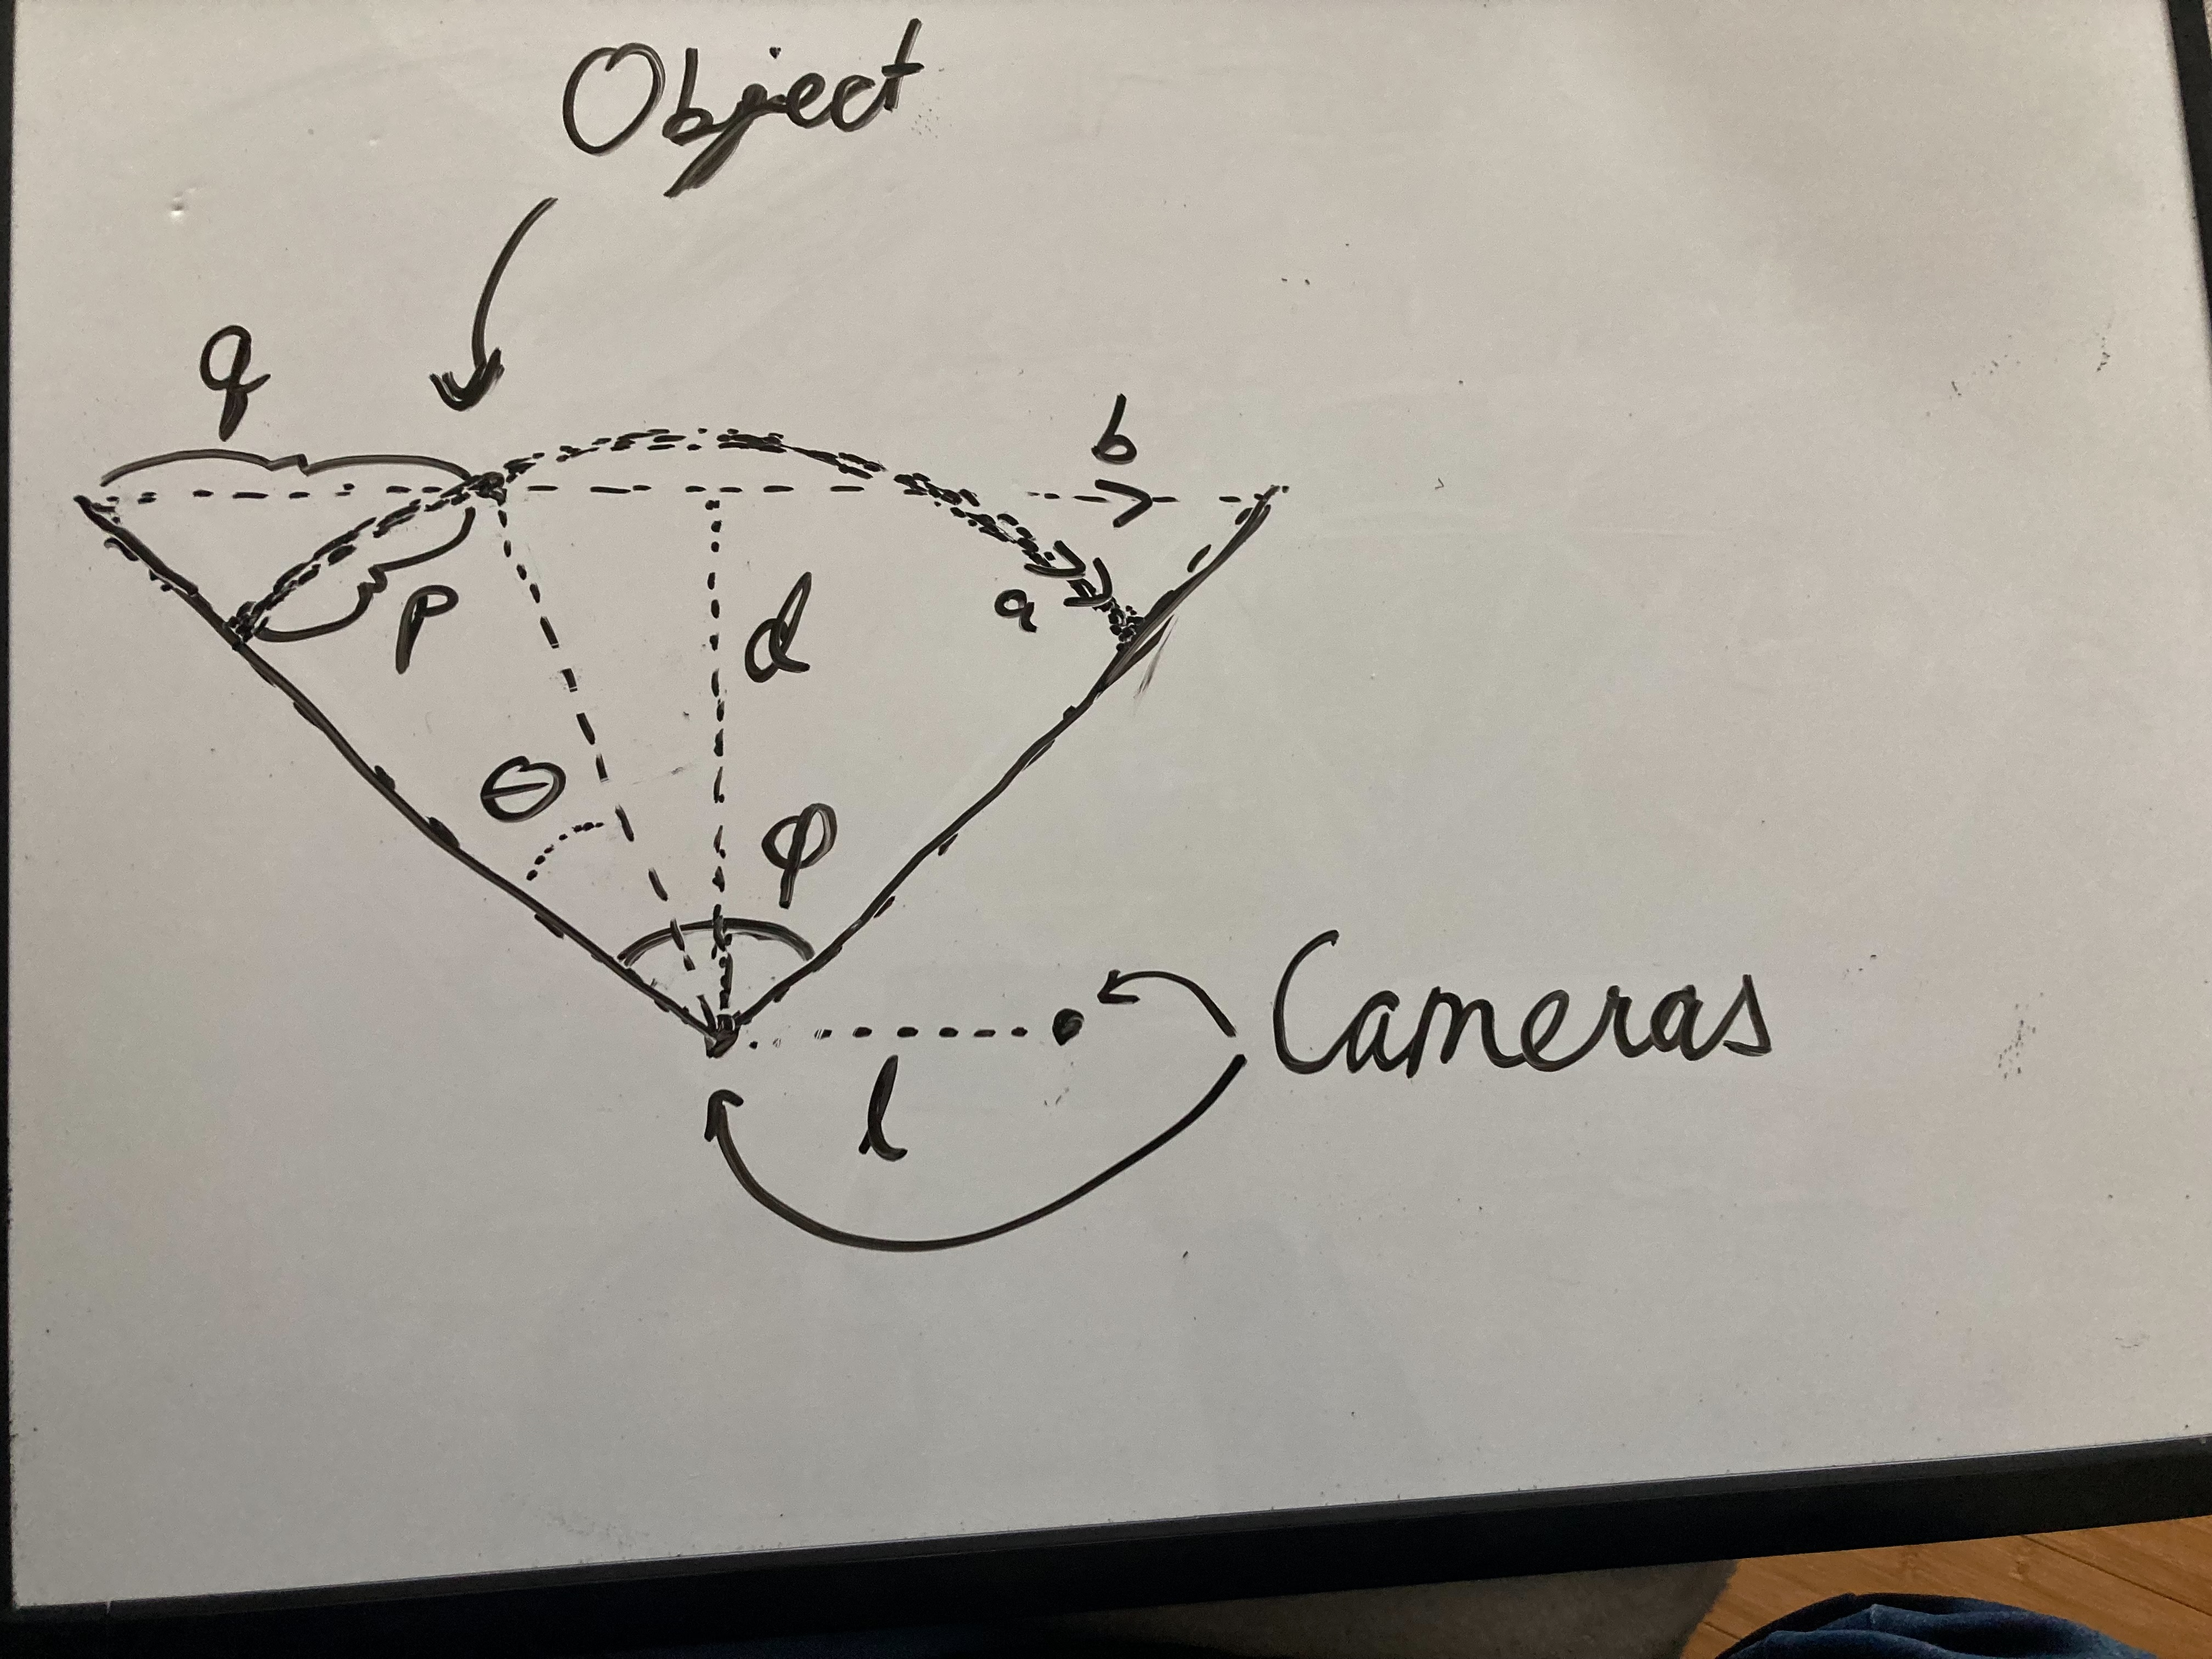
\includegraphics[width=10cm]{Phase I/variable_defs.jpg}
    \caption{Variable definitions}
 
\end{figure}
\newline \newline
In words, $\phi$ is the angle of the camera's total field of vision, and $\theta$ is the angle the object makes with the camera and the left boundary of the field of vision. The distance between the cameras is $l$, the circular arc through the object and centered at the camera is labelled $a$, and the segment through the object and parallel to the cameras is labelled $b$. The distance from the camera to segment $b$ is $d$. The proportion of segment $b$ to the left of the object is denoted $q$, and the proportion of the arc $a$ to the left of the object is denoted $p$. \newline \newline
Importantly, $q$ and $p$ represent the proportion of the linear or curved (respectively) field of vision to the left of the object. This means that they are both numbers between 0 and 1. From this, we immediately see that $p = \frac{\theta}{\phi}$. We also see that trigonometry will be instrumental in creating our algorithm to estimate depth. \newline \newline
Now, we incorporate a binocular shift. The following image shows how $\Delta q = \frac{l}{\alpha \cdot d}$, where $\Delta q$  is the difference in $q$ from each camera's perspective, and $\alpha$ is a constant that can be approximated by $2 \cdot tan(\frac{\phi}{2})$. Also note that the quantities labelled $q$ and $q - \Delta q$ appear to represent lengths, when they actually represent proportions (I wasn't sure how to show this visually). This can be done by setting the total length of segment $b$ to 1. 
\begin{figure}[htp]
    \centering
    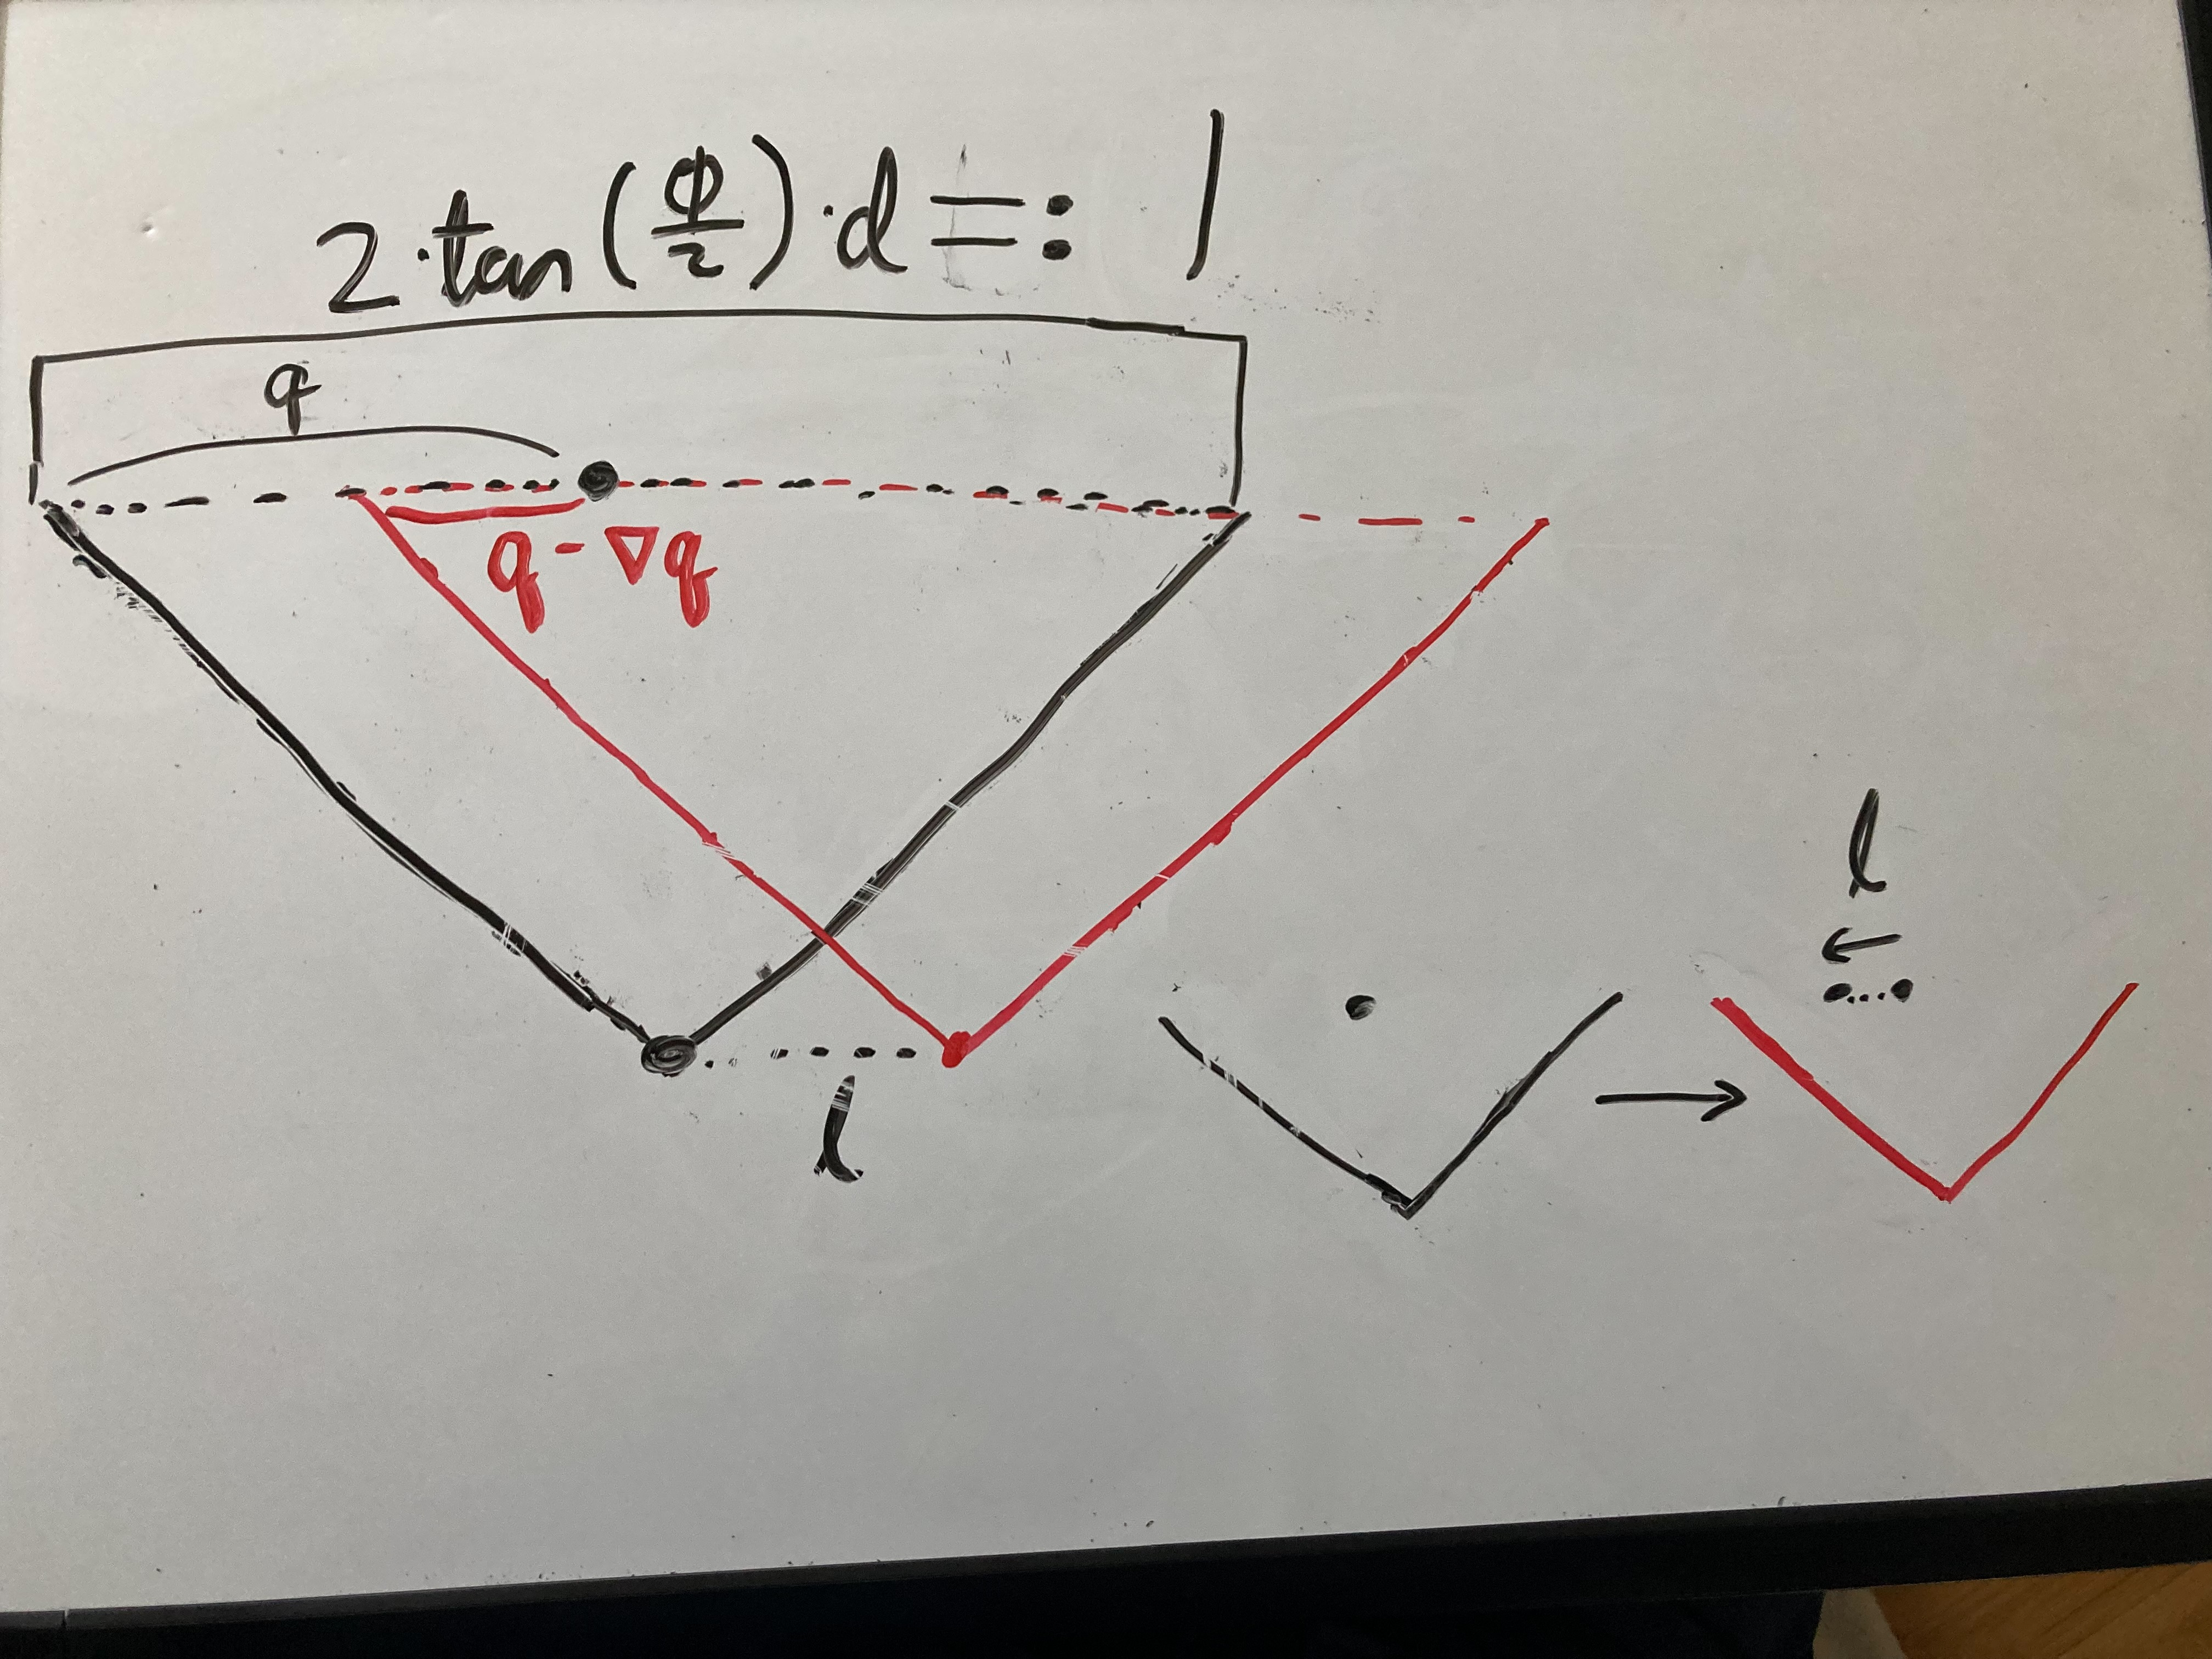
\includegraphics[width=10cm]{Phase I/deltaq.jpg}
    \caption{Finding $\Delta q$}
\end{figure}
\newline \newline
Unfortunately, $q$ is not easily readable from the images seen by the pictures. Instead, I assumed that cameras would compress objects in a circular arc (because objects that are the same distance from the camera would "shrink" the same amount"). This is analogous to how a moving car appears to a stationary observer: if the car moves in a straight line, it traverses across the observer's field of vision fastest when it's motion is perpendicular to the observer's gaze. However, if the car moves around the observer in a circle, it traverses the observer's field of vision at a constant rate. \newline \newline
This raises a challenge, as $d$ and $l$ are related to $q$, while $p$ is the proportion that is readable from the camera image (distance on the left/total width of image). Thus, connecting $p$ and $q$ would "solve" the problem. The connection with $p$ and $q$ is as shown in the following diagram (next page): \newline \newline
Thus, to find an estimate of depth given binocular input, a computer would take a couple "ground truth" examples to find $l$ and $\phi$. Then, given a new object, one could easily find $p$, then find $\theta$, then calculate $q$. After doing this for both images, the difference between the two values of $q$ could then be used to find $d$. 

\section{Next phases}
Some brief comments are that I want to include a few fully connected layers in the CNN early on so that the model will be able to incorporate global differences between the two angles of the scene.

\begin{figure}[htp]
    \centering
    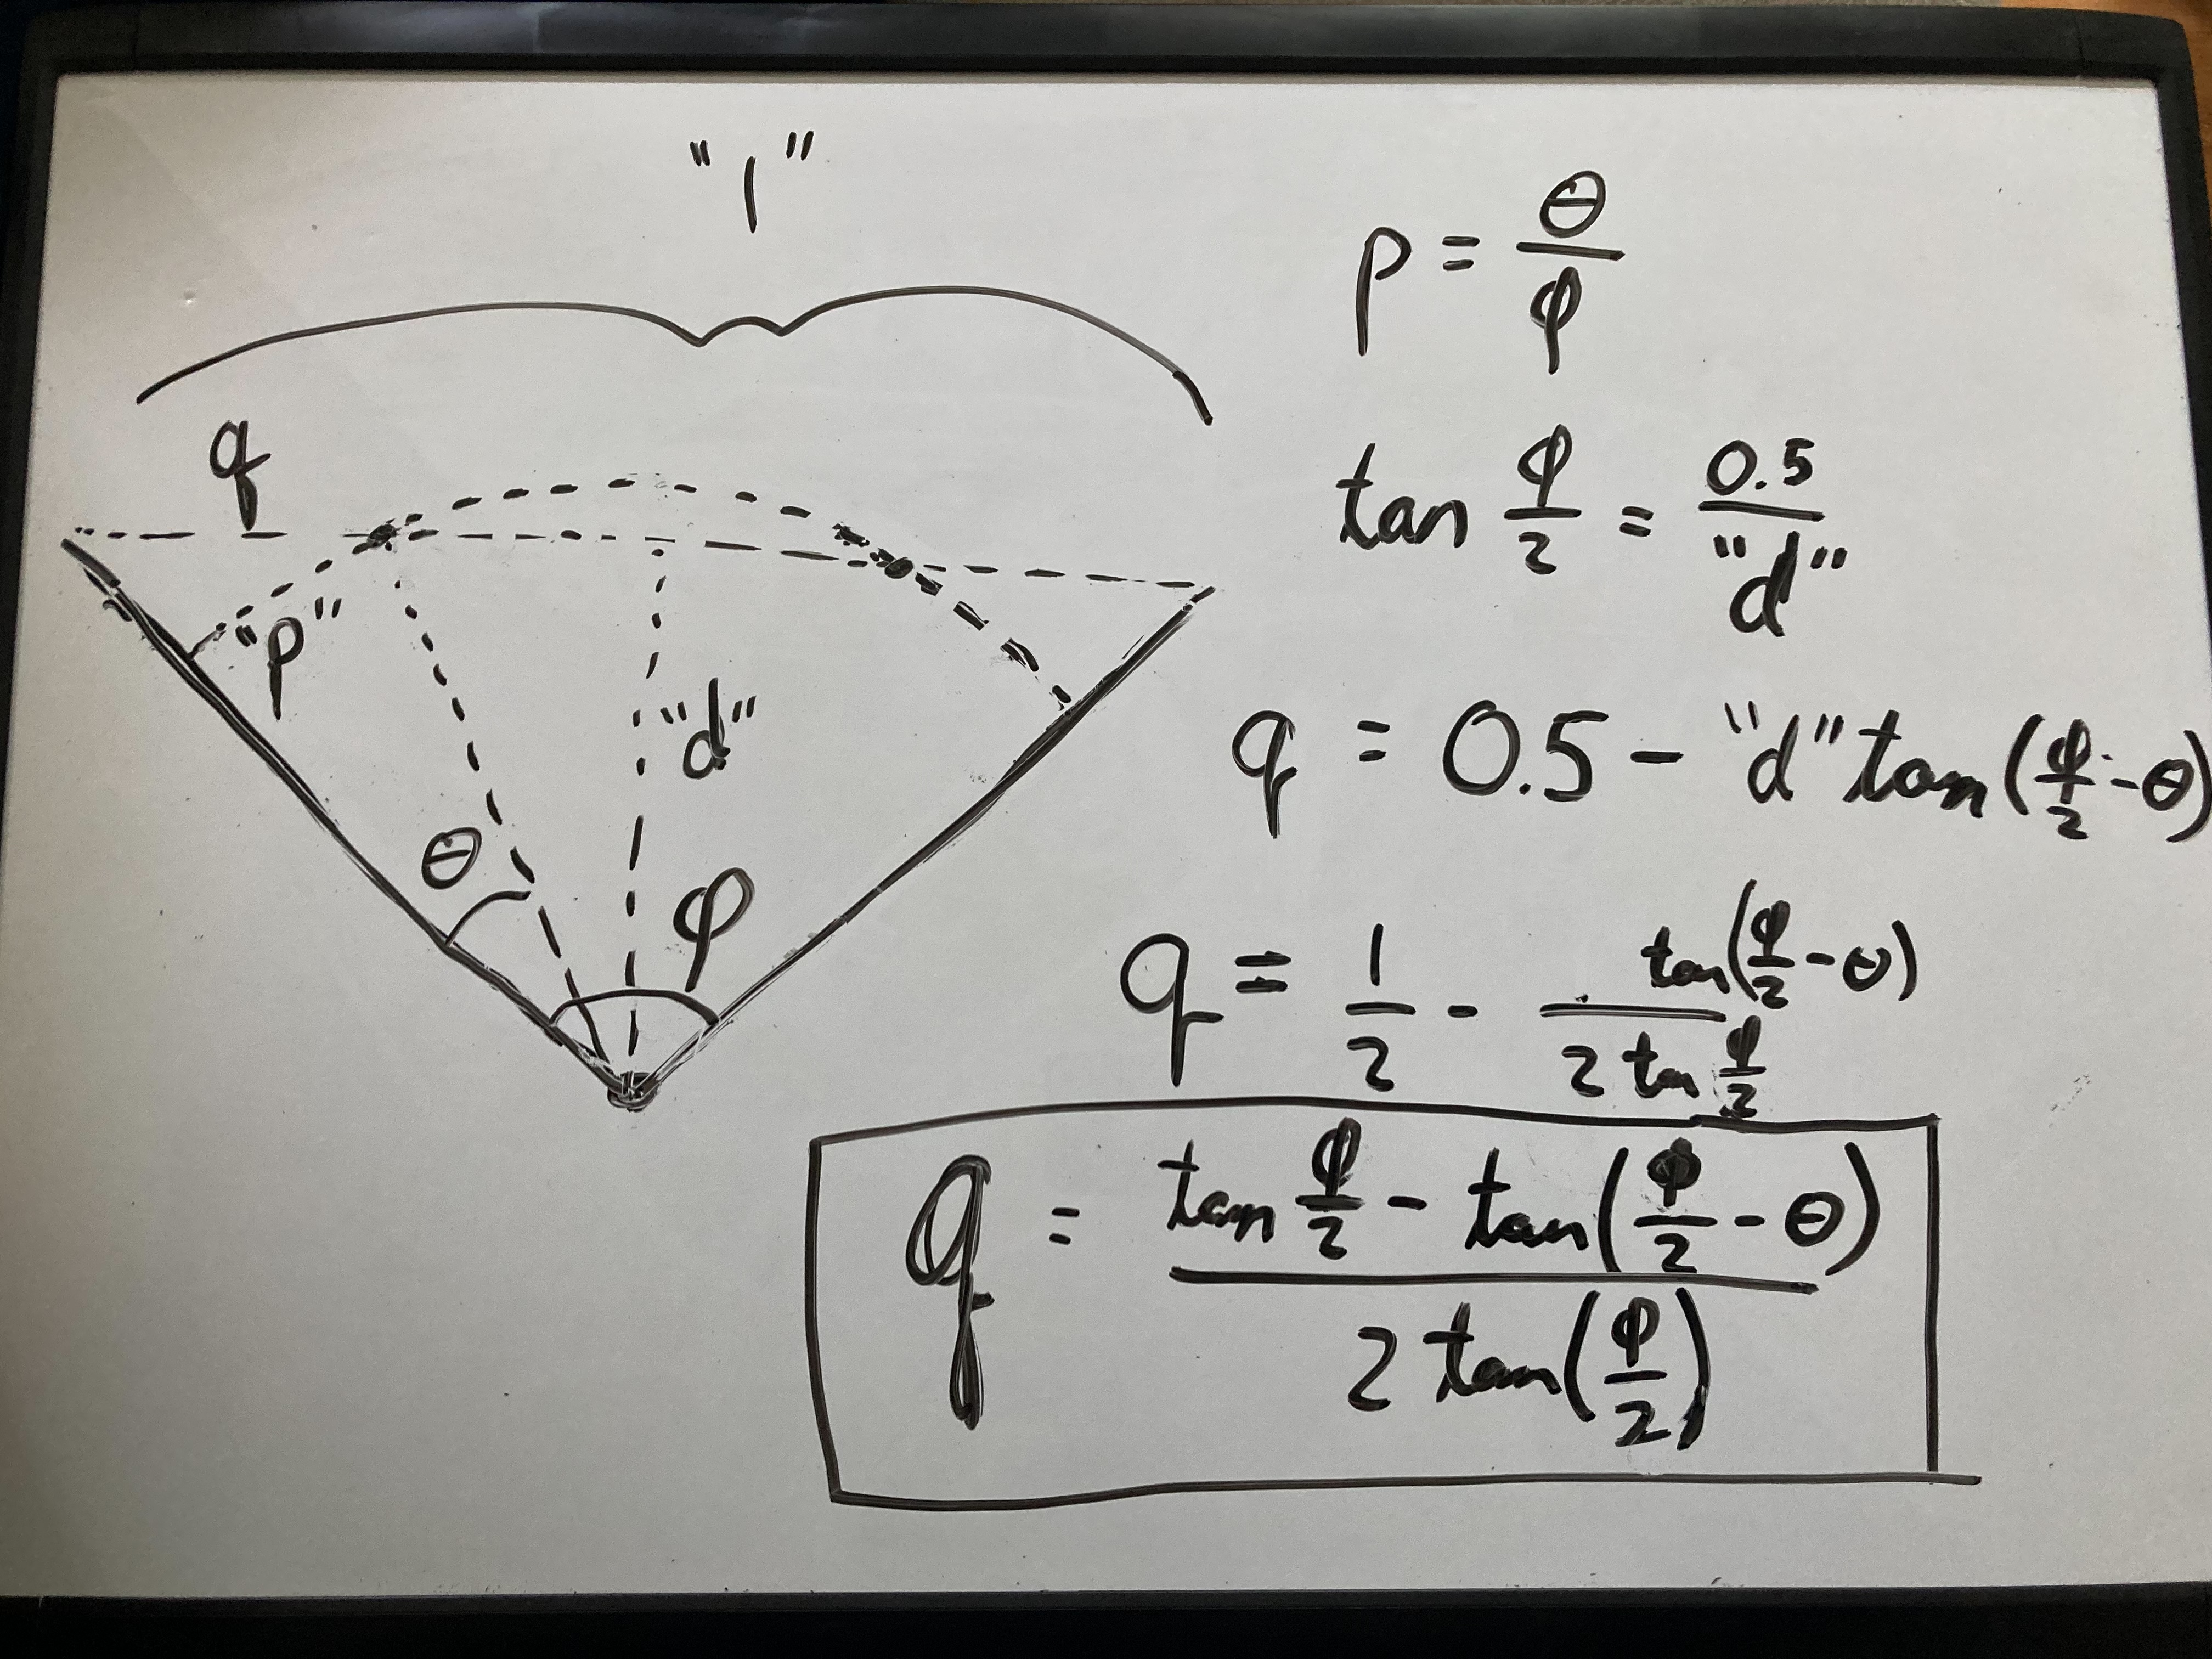
\includegraphics[width=12cm]{Phase I/qfromp.jpg}
    \caption{Finding q from p}
\end{figure}


\end{document}
